
%% bare_conf.tex
%% V1.4b
%% 2015/08/26
%% by Michael Shell
%% See:
%% http://www.michaelshell.org/
%% for current contact information.
%%
%% This is a skeleton file demonstrating the use of IEEEtran.cls
%% (requires IEEEtran.cls version 1.8b or later) with an IEEE
%% conference paper.
%%
%% Support sites:
%% http://www.michaelshell.org/tex/ieeetran/
%% http://www.ctan.org/pkg/ieeetran
%% and
%% http://www.ieee.org/

%%*************************************************************************
%% Legal Notice:
%% This code is offered as-is without any warranty either expressed or
%% implied; without even the implied warranty of MERCHANTABILITY or
%% FITNESS FOR A PARTICULAR PURPOSE! 
%% User assumes all risk.
%% In no event shall the IEEE or any contributor to this code be liable for
%% any damages or losses, including, but not limited to, incidental,
%% consequential, or any other damages, resulting from the use or misuse
%% of any information contained here.
%%
%% All comments are the opinions of their respective authors and are not
%% necessarily endorsed by the IEEE.
%%
%% This work is distributed under the LaTeX Project Public License (LPPL)
%% ( http://www.latex-project.org/ ) version 1.3, and may be freely used,
%% distributed and modified. A copy of the LPPL, version 1.3, is included
%% in the base LaTeX documentation of all distributions of LaTeX released
%% 2003/12/01 or later.
%% Retain all contribution notices and credits.
%% ** Modified files should be clearly indicated as such, including  **
%% ** renaming them and changing author support contact information. **
%%*************************************************************************


% *** Authors should verify (and, if needed, correct) their LaTeX system  ***
% *** with the testflow diagnostic prior to trusting their LaTeX platform ***
% *** with production work. The IEEE's font choices and paper sizes can   ***
% *** trigger bugs that do not appear when using other class files.       ***                          ***
% The testflow support page is at:
% http://www.michaelshell.org/tex/testflow/



\documentclass[conference]{IEEEtran}
% Some Computer Society conferences also require the compsoc mode option,
% but others use the standard conference format.
%
% If IEEEtran.cls has not been installed into the LaTeX system files,
% manually specify the path to it like:
% \documentclass[conference]{../sty/IEEEtran}





% Some very useful LaTeX packages include:
% (uncomment the ones you want to load)


% *** MISC UTILITY PACKAGES ***
%
%\usepackage{ifpdf}
% Heiko Oberdiek's ifpdf.sty is very useful if you need conditional
% compilation based on whether the output is pdf or dvi.
% usage:
% \ifpdf
%   % pdf code
% \else
%   % dvi code
% \fi
% The latest version of ifpdf.sty can be obtained from:
% http://www.ctan.org/pkg/ifpdf
% Also, note that IEEEtran.cls V1.7 and later provides a builtin
% \ifCLASSINFOpdf conditional that works the same way.
% When switching from latex to pdflatex and vice-versa, the compiler may
% have to be run twice to clear warning/error messages.



\usepackage{float}
 \usepackage{booktabs}

% *** CITATION PACKAGES ***
%
\usepackage{cite}
% cite.sty was written by Donald Arseneau
% V1.6 and later of IEEEtran pre-defines the format of the cite.sty package
% \cite{} output to follow that of the IEEE. Loading the cite package will
% result in citation numbers being automatically sorted and properly
% "compressed/ranged". e.g., [1], [9], [2], [7], [5], [6] without using
% cite.sty will become [1], [2], [5]--[7], [9] using cite.sty. cite.sty's
% \cite will automatically add leading space, if needed. Use cite.sty's
% noadjust option (cite.sty V3.8 and later) if you want to turn this off
% such as if a citation ever needs to be enclosed in parenthesis.
% cite.sty is already installed on most LaTeX systems. Be sure and use
% version 5.0 (2009-03-20) and later if using hyperref.sty.
% The latest version can be obtained at:
% http://www.ctan.org/pkg/cite
% The documentation is contained in the cite.sty file itself.






% *** GRAPHICS RELATED PACKAGES ***
%
\ifCLASSINFOpdf
  \usepackage[pdftex]{graphicx}
  % declare the path(s) where your graphic files are
  % \graphicspath{{../pdf/}{../jpeg/}}
  % and their extensions so you won't have to specify these with
  % every instance of \includegraphics
  % \DeclareGraphicsExtensions{.pdf,.jpeg,.png}
\else
  % or other class option (dvipsone, dvipdf, if not using dvips). graphicx
  % will default to the driver specified in the system graphics.cfg if no
  % driver is specified.
  \usepackage[dvips]{graphicx}
  % declare the path(s) where your graphic files are
  % \graphicspath{{../eps/}}
  % and their extensions so you won't have to specify these with
  % every instance of \includegraphics
  % \DeclareGraphicsExtensions{.eps}
\fi
% graphicx was written by David Carlisle and Sebastian Rahtz. It is
% required if you want graphics, photos, etc. graphicx.sty is already
% installed on most LaTeX systems. The latest version and documentation
% can be obtained at: 
% http://www.ctan.org/pkg/graphicx
% Another good source of documentation is "Using Imported Graphics in
% LaTeX2e" by Keith Reckdahl which can be found at:
% http://www.ctan.org/pkg/epslatex
%
% latex, and pdflatex in dvi mode, support graphics in encapsulated
% postscript (.eps) format. pdflatex in pdf mode supports graphics
% in .pdf, .jpeg, .png and .mps (metapost) formats. Users should ensure
% that all non-photo figures use a vector format (.eps, .pdf, .mps) and
% not a bitmapped formats (.jpeg, .png). The IEEE frowns on bitmapped formats
% which can result in "jaggedy"/blurry rendering of lines and letters as
% well as large increases in file sizes.
%
% You can find documentation about the pdfTeX application at:
% http://www.tug.org/applications/pdftex





% *** MATH PACKAGES ***
%
\usepackage{amsmath}
% A popular package from the American Mathematical Society that provides
% many useful and powerful commands for dealing with mathematics.
%
% Note that the amsmath package sets \interdisplaylinepenalty to 10000
% thus preventing page breaks from occurring within multiline equations. Use:
%\interdisplaylinepenalty=2500
% after loading amsmath to restore such page breaks as IEEEtran.cls normally
% does. amsmath.sty is already installed on most LaTeX systems. The latest
% version and documentation can be obtained at:
% http://www.ctan.org/pkg/amsmath





% *** SPECIALIZED LIST PACKAGES ***
%
%\usepackage{algorithmic}
% algorithmic.sty was written by Peter Williams and Rogerio Brito.
% This package provides an algorithmic environment fo describing algorithms.
% You can use the algorithmic environment in-text or within a figure
% environment to provide for a floating algorithm. Do NOT use the algorithm
% floating environment provided by algorithm.sty (by the same authors) or
% algorithm2e.sty (by Christophe Fiorio) as the IEEE does not use dedicated
% algorithm float types and packages that provide these will not provide
% correct IEEE style captions. The latest version and documentation of
% algorithmic.sty can be obtained at:
% http://www.ctan.org/pkg/algorithms
% Also of interest may be the (relatively newer and more customizable)
% algorithmicx.sty package by Szasz Janos:
% http://www.ctan.org/pkg/algorithmicx




% *** ALIGNMENT PACKAGES ***
%
%\usepackage{array}
% Frank Mittelbach's and David Carlisle's array.sty patches and improves
% the standard LaTeX2e array and tabular environments to provide better
% appearance and additional user controls. As the default LaTeX2e table
% generation code is lacking to the point of almost being broken with
% respect to the quality of the end results, all users are strongly
% advised to use an enhanced (at the very least that provided by array.sty)
% set of table tools. array.sty is already installed on most systems. The
% latest version and documentation can be obtained at:
% http://www.ctan.org/pkg/array


% IEEEtran contains the IEEEeqnarray family of commands that can be used to
% generate multiline equations as well as matrices, tables, etc., of high
% quality.




% *** SUBFIGURE PACKAGES ***
\ifCLASSOPTIONcompsoc
  \usepackage[caption=false,font=normalsize,labelfont=sf,textfont=sf]{subfig}
\else
  \usepackage[caption=false,font=footnotesize]{subfig}
\fi
% subfig.sty, written by Steven Douglas Cochran, is the modern replacement
% for subfigure.sty, the latter of which is no longer maintained and is
% incompatible with some LaTeX packages including fixltx2e. However,
% subfig.sty requires and automatically loads Axel Sommerfeldt's caption.sty
% which will override IEEEtran.cls' handling of captions and this will result
% in non-IEEE style figure/table captions. To prevent this problem, be sure
% and invoke subfig.sty's "caption=false" package option (available since
% subfig.sty version 1.3, 2005/06/28) as this is will preserve IEEEtran.cls
% handling of captions.
% Note that the Computer Society format requires a larger sans serif font
% than the serif footnote size font used in traditional IEEE formatting
% and thus the need to invoke different subfig.sty package options depending
% on whether compsoc mode has been enabled.
%
% The latest version and documentation of subfig.sty can be obtained at:
% http://www.ctan.org/pkg/subfig




% *** FLOAT PACKAGES ***
%
%\usepackage{fixltx2e}
% fixltx2e, the successor to the earlier fix2col.sty, was written by
% Frank Mittelbach and David Carlisle. This package corrects a few problems
% in the LaTeX2e kernel, the most notable of which is that in current
% LaTeX2e releases, the ordering of single and double column floats is not
% guaranteed to be preserved. Thus, an unpatched LaTeX2e can allow a
% single column figure to be placed prior to an earlier double column
% figure.
% Be aware that LaTeX2e kernels dated 2015 and later have fixltx2e.sty's
% corrections already built into the system in which case a warning will
% be issued if an attempt is made to load fixltx2e.sty as it is no longer
% needed.
% The latest version and documentation can be found at:
% http://www.ctan.org/pkg/fixltx2e


%\usepackage{stfloats}
% stfloats.sty was written by Sigitas Tolusis. This package gives LaTeX2e
% the ability to do double column floats at the bottom of the page as well
% as the top. (e.g., "\begin{figure*}[!b]" is not normally possible in
% LaTeX2e). It also provides a command:
%\fnbelowfloat
% to enable the placement of footnotes below bottom floats (the standard
% LaTeX2e kernel puts them above bottom floats). This is an invasive package
% which rewrites many portions of the LaTeX2e float routines. It may not work
% with other packages that modify the LaTeX2e float routines. The latest
% version and documentation can be obtained at:
% http://www.ctan.org/pkg/stfloats
% Do not use the stfloats baselinefloat ability as the IEEE does not allow
% \baselineskip to stretch. Authors submitting work to the IEEE should note
% that the IEEE rarely uses double column equations and that authors should try
% to avoid such use. Do not be tempted to use the cuted.sty or midfloat.sty
% packages (also by Sigitas Tolusis) as the IEEE does not format its papers in
% such ways.
% Do not attempt to use stfloats with fixltx2e as they are incompatible.
% Instead, use Morten Hogholm'a dblfloatfix which combines the features
% of both fixltx2e and stfloats:
%
% \usepackage{dblfloatfix}
% The latest version can be found at:
% http://www.ctan.org/pkg/dblfloatfix




% *** PDF, URL AND HYPERLINK PACKAGES ***
%
\usepackage{url}
% url.sty was written by Donald Arseneau. It provides better support for
% handling and breaking URLs. url.sty is already installed on most LaTeX
% systems. The latest version and documentation can be obtained at:
% http://www.ctan.org/pkg/url
% Basically, \url{my_url_here}.




% *** Do not adjust lengths that control margins, column widths, etc. ***
% *** Do not use packages that alter fonts (such as pslatex).         ***
% There should be no need to do such things with IEEEtran.cls V1.6 and later.
% (Unless specifically asked to do so by the journal or conference you plan
% to submit to, of course. )


% correct bad hyphenation here
\hyphenation{op-tical net-works semi-conduc-tor }

\IEEEoverridecommandlockouts
\begin{document}
%
% paper title
% Titles are generally capitalized except for words such as a, an, and, as,
% at, but, by, for, in, nor, of, on, or, the, to and up, which are usually
% not capitalized unless they are the first or last word of the title.
% Linebreaks \\ can be used within to get better formatting as desired.
% Do not put math or special symbols in the title.
\title{Selective Data Transfer from DRAMs for CNNs }


% author names and affiliations
% use a multiple column layout for up to three different
% affiliations
%	\author{\IEEEauthorblockN{Michael Shell}
%	\IEEEauthorblockA{School of Electrical and\\Computer Engineering\\
%	Georgia Institute of Technology\\
%	Atlanta, Georgia 30332--0250\\
%	Email: http://www.michaelshell.org/contact.html}
%	\and
%	\IEEEauthorblockN{Homer Simpson}
%	\IEEEauthorblockA{Twentieth Century Fox\\
%	Springfield, USA\\
%	Email: homer@thesimpsons.com}
%	\and
%	\IEEEauthorblockN{James Kirk\\ and Montgomery Scott}
%	\IEEEauthorblockA{Starfleet Academy\\
%	San Francisco, California 96678--2391\\
%	Telephone: (800) 555--1212\\
%	Fax: (888) 555--1212}}

\author{\IEEEauthorblockN{Anaam Ansari\IEEEauthorrefmark{1}\IEEEauthorrefmark{2}\thanks{\IEEEauthorrefmark{2}aaansari@scu.edu}, 
Tokunbo Ogunfunmi\IEEEauthorrefmark{1}\IEEEauthorrefmark{3}\thanks{\IEEEauthorrefmark{3}togunfunmi@scu.edu}}
\IEEEauthorblockA{\IEEEauthorrefmark{1}Department of Electrical Engineering\\
Santa Clara University,
Santa Clara, California 95053}
}


% conference papers do not typically use \thanks and this command
% is locked out in conference mode. If really needed, such as for
% the acknowledgment of grants, issue a \IEEEoverridecommandlockouts
% after \documentclass

% for over three affiliations, or if they all won't fit within the width
% of the page, use this alternative format:
% 
%\author{\IEEEauthorblockN{Michael Shell\IEEEauthorrefmark{1},
%Homer Simpson\IEEEauthorrefmark{2},
%James Kirk\IEEEauthorrefmark{3}, 
%Montgomery Scott\IEEEauthorrefmark{3} and
%Eldon Tyrell\IEEEauthorrefmark{4}}
%\IEEEauthorblockA{\IEEEauthorrefmark{1}School of Electrical and Computer Engineering\\
%Georgia Institute of Technology,
%Atlanta, Georgia 30332--0250\\ Email: see http://www.michaelshell.org/contact.html}
%\IEEEauthorblockA{\IEEEauthorrefmark{2}Twentieth Century Fox, Springfield, USA\\
%Email: homer@thesimpsons.com}
%\IEEEauthorblockA{\IEEEauthorrefmark{3}Starfleet Academy, San Francisco, California 96678-2391\\
%Telephone: (800) 555--1212, Fax: (888) 555--1212}
%\IEEEauthorblockA{\IEEEauthorrefmark{4}Tyrell Inc., 123 Replicant Street, Los Angeles, California 90210--4321}}




% use for special paper notices
%\IEEEspecialpapernotice{(Invited Paper)}




% make the title area
\maketitle

% As a general rule, do not put math, special symbols or citations
% in the abstract
\begin{abstract}
Convolutional Neural Networks (CNN) have changed the direction of image and speech signal processing. They have becoming prolific in applications such as self driving cars and voice assitants like Siri and Alexa. Since the success of AlexNet, many deep learning networks like GoogleNet, ResidualNet etc have been introduced. These networks are highly competent in image classification however, they are very large in size and have a lot of parameters, for example, AlexNet has 60M parameters\cite{krizhevsky2012imagenet}. On-Off chip data transfer is a great engineering challenge that needs to be addressed while implementing CNN in hardware. Hardware Acceleration and parallelization are constrained by energy cost of reading and writing data from memory. For one forward pass during inference, one image needs to go through to all the CNN layers and be classified into a softmax determined category. During this process, the memory bandwidth is used by three types of payloads that need to be moved on and off-chip - input image, intermediate feature maps, and filter weights. This research is focused on reducing weight-related memory traffic that occurs between off-chip memory and on-chip buffers. In this paper, we propose a technique named `weight sharing selective transfer' (WS-ST) that uses processing in-memory architecture to selectively transfer weights from the DRAM memory structure to the computation unit. We observe a $30\%$ decrease in memory transfer traffic compared to a non-selective approach for AlexNet. We achieve this by implementing a selector logic in the DRAM itself. This logic helps us select the weights that need to be updated and avoid the transfer if the weight value is the same. 
 


\end{abstract}

\begin{IEEEkeywords}
CNN, selective data-transfer, AlexNet
\end{IEEEkeywords}
% no keywords




% For peer review papers, you can put extra information on the cover
% page as needed:
% \ifCLASSOPTIONpeerreview
% \begin{center} \bfseries EDICS Category: 3-BBND \end{center}
% \fi
%
% For peerreview papers, this IEEEtran command inserts a page break and
% creates the second title. It will be ignored for other modes.
\IEEEpeerreviewmaketitle



\section{Introduction}
Deep Learning is an emerging technology that is taking over new areas of application. Deep learning networks are evolving to be larger and more complex than ever\cite{he2016deep, szegedy2015going}. The hardware technology is constantly playing catch up to keep up with the sophistication we see in the algorithmic innovation of CNNs. Power and computation complexity are the challenges that need to be addressed as these networks keep getting larger and more complex. 
Hardware acceleration on FPGAs\cite{Lacey2016} and ASICs is gaining momentum as they prove to be more energy efficient and portable than GPUs for inference\cite{Fowers:2012:PEC:2145694.2145704} \cite{sze2017efficient}.  

Although hardware acceleration on FPGAs is lucrative, there are unique engineering challenges that limit this area. The major challenges include memory related traffic management, computation complexity, and complex parallelization. The memory bandwidth directly contributes to energy consumption as the movement of data from the DRAM is the most costly of all operations \cite{han2016eie}.

\begin{table}[!ht]
\centering
\caption{Energy Cost of DRAM access compared to other operations\cite{han2016eie}}
\label{energy}
\begin{tabular}{ccc}
\hline
\textbf{Operation} & \textbf{Energy (pJ)} & \textbf{Relative Cost} \\ \hline
32 bit int ADD     & 0.1                  & 1                      \\
32 bit float ADD   & 0.9                  & 9                      \\
32 bit int MULT    & 3.1                  & 31                     \\
32 bit float MULT  & 3.7                  & 37                     \\
32 bit 32KB SRAM   & 5                    & 50                     \\
32 bit DRAM        & 640                  & 6400                   \\ \hline
\end{tabular}
\end{table}


There are many popular dense CNN Accelerator designs for FPGAs \cite{chakradhar2010dynamically,zhang2015optimizing,Eyeriss}.
The techniques commonly used in dense architectures are loop blocking, loop unrolling and data stationary operations and data reuse. 

In contrast to this, there has been new research in adapting sparse models and sparse computation in CNNs. Pruning techniques have proved that smaller models gain a lot in terms of performance and energy efficiency at a slight bearable cost in accuracy \cite{zhu2017prune, DBLP:journals/corr/abs-1708-04485, han2016eie, liu2018efficient, mao2017exploring, han2016dsd}.

In this work, we contribute the following:
\begin{itemize}
\item We analyze the redundancy in the filter weight kernels that are used in convolutional layers and fully connected layers after they are compressed using a technique called weight technique called `weight sharing'. 
\item We model a DRAM that is capable of performing simple logic operations like compare or XOR.
\item The modified DRAM helps us reduce the weight transfer from DRAM and main computational unit. 
\end{itemize}

\section{Motivation}
Latest techniques like pruning and sparse computation have illustrated the benefits of reducing the model size. 
These compressed models eliminate the need to store full sized models with all the parameters and do not hurt the original accuracy\cite{li2016pruning}. Another way to minimize the storage of input and weights in the main memory is quantization. \cite{wu2016quantized, jouppi2017datacenter, HSong_lecture}. Although, quantization leads to a deterioration of accuracy a balance can be achieved between maintaining a low enough precision and tolerable accuracy. 


Techniques to compress the network such as pruning lead to sparse networks and generate associative data as it is stored in other irregular formats. However, processing irregular networks is beyond the scope of this research. 

There has also been an interest in the processing-in-memory (PIM) architecture and near-data-computation (NDC) to reduce the memory transfer from main memory to host processing unit\cite{kim2016neurocube, gao2017tetris, jiang2017xnor, chi2016prime}. Due to the popularity of stacked DRAMs such as HMC and HBM \cite{black2013hybrid, standard2013high}. These DRAM architectures provide a promising throughput and latency performance. The through silicon vias  (TSVs) have a higher bandwidth. 

In this research, we exploit the redundancy of weights that is a result of a process called `weight sharing'\cite{han2015deep}. We design a weight selector logic to selectively send only the weights that are different than the ones used in the prior output f-map calculation. 

Weight sharing can reduce the number of parameters drastically in a network \cite{han2016eie}. They can be presented by using a small number of bits hence, there are a limited number of values the weights can assume. As a result of sharing, many values are repeated across different kernels. This is the redundancy we will exploit.

To do this, we aim to have a processing-in-memory architecture  using stacked DRAM. The weight selector we design will bring in chunks of weight from the weight payload into registers near the data memory. Then the comparison of previous weight to the subsequent weight takes place and a decision is made. If the weights are found to be the same no action is taken and if they are different we update them in the buffer. 

%(if time permits)
%
%In order to have a symmetry in architecture we will also implement a selection scheme on the output of the CNN layers. This will help us improve the offload the data write and read to the main memory. Thus contributing to the overall of reduction in memory bandwidth. 



\section{Analysis}

In this section, we explain the rationale and analysis that lies at the foundation of our approach. The following analysis gives an insight about the superfluous repetitiveness of the shared weights. We perform this analysis on many levels of granularity i.e. bit precisions such as 1 bit, 4bit (a nibble) and 8bit (a byte). Studying the redundancy at various precision levels helps us select a bus size for the DRAM that will be best suited for our architecture and design. For this analysis, we use pre-trained AlexNet weights as our source for weight\cite{alexnet_matlab}.

\subsection{Weight Sharing} 
As a part of our analysis, we first convert the AlexNet weights into a shared format. Weight sharing is a pruning technique that is used to overcome a network being over-fitted. It was discovered mainly to combat over-fitting a network however, it helps  compress a model too \cite{zhu2017prune, li2016pruning, han2015deep, anwar2017structured}. A compressed model is retrained with the shared weights. Weight sharing makes retraining very efficient and also helps the models be more generalized and less over-fitted. 

Making weights assume same values is of strategic value from an algorithmic point of view as well as the engineering point of view. We covert the weights to a 4 bit precision and 8 bit precision. This gives us 16 and 256 weight values respectively. Once the 16 and 256 weights are shared among all the layers (Convolutional and Fully connected layers) we implement the selection process. 


\subsection{Selective PassThrough}
After the weights are shared, we can design a selection logic to pass through weights that need to be updated as opposed to writing all the weights to on chip memory without dealing with the redundancy. The logic to select weights from the weight payload is described in figure \ref{sel}. We compare the subsequent weight with the previous weight and if it is found to be different we update it on chip if not we do nothing. We can choose to compare at any desired granularity.

\begin{figure}[!ht]
\centering
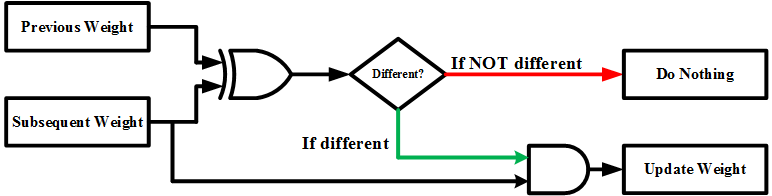
\includegraphics[width=3.5in]{selector}
\caption{Weight selector Logic}
\label{sel}
\end{figure}

\subsection{Redundancy Analysis}
In the matlab analysis, we evaluate the redundancy in AlexNet weights after compressing them using weight sharing. 
The analysis process is as follows and entails the following experiments.
\begin{itemize}
\item Comparing 4 bit weights for 16 shared weights at the granularity level of 4 bits. 

\item Comparing 4 bit weights for 16 shared weights at the granularity level of 1 bit. 

\item Comparing 8 bit weights for 256 shared weights at the granularity level of 8 bits. 

\item Comparing 8 bit weights for 256 shared weights at the granularity level of 1 bit. 
\end{itemize}

We choose 4bit and 8 bit weight precisions as 4bit of weight precision using dense sparse dense (DSD) training process in \cite{han2016dsd} does very well in terms of accuracy while also compressing it to a great degree. Looking at results in figures \ref{Conv_Red} and \ref{FC_Red}, we see that 
we are able to find more redundancy with smaller granularity. Both figures \ref{Con_Red_bits} and \ref{Con_Red_8_bits} in figure \ref{Conv_Red} show us that we can eliminate a large number of weight bits that are common between the batch of previous weight and the subsequent weight that needs to be sent to the chip. For fully connected layers, we see that in figures \ref{FC_Red_bits} and  \ref{FC_Red_8bits_256lev_bits} we see the same trend. However, this is a very low level of granularity and will impose more challenges for a controller than being useful. One bit granularity will also provide a slow rate of transfer. Thus, the real choice is between 4 bit and 8 bit of granularity. Going to a higher granularity will increase the weight value levels and be in vain. Looking at figures \ref{Con_Red}, \ref{Con_Red_8}, \ref{FC_Red_4bits} and \ref{FC_Red_8bits_256lev}, we can see that 4 bit weights provide the right amount granularity and weight levels. 

Looking at the result, we chosoe the 4 bit granularity as it exploits a good amount redundancy while being manageable in terms of hardware engineering. The savings with 4 bit weights and 4 bit granularity is described in table \ref{Red_Anal}.

\begin{table*}[!ht]
\centering
\caption{Redundancy Analysis for 4 bit weights with 4 bit granularity}
\label{Red_Anal}
\begin{tabular}{ccccccccc}
\hline
Layer & height    & width    & c   & kernels & total weights & selective weights  & difference & \% Improvement \\ \hline
conv1 & 11   & 11   & 3   & 96      & 34848         & 23092             & 11756      & 33.74          \\
conv2 & 5    & 5    & 48  & 256     & 307200        & 97045             & 210155     & 68.41          \\
conv3 & 3    & 3    & 256 & 384     & 884736        & 446751            & 437985     & 49.50          \\
conv4 & 3    & 3    & 192 & 384     & 663552        & 312345             & 351207     & 52.93          \\
conv5 & 3    & 3    & 192 & 256     & 442368        & 239363             & 203005     & 45.89          \\
fc1   & 4096 & 9216 & 1   & 1       & 37748736      & 25618179         & 12130557   & 32.14          \\
fc2   & 4096 & 4096 & 1   & 1       & 16777216      & 11661838          & 5115378    & 30.49          \\
fc3   & 1000 & 4096 & 1   & 1       & 4096000       & 4096000           & 0          & 0              \\ \hline
total &      &      &     &         & 60954656      & 42494613          & 18460043   & 30.28          \\ \hline
\end{tabular}
\end{table*}

\begin{figure*}[]
\centering
\begin{tabular}{cc}

\subfloat[4bit weight, 4bit granularity]{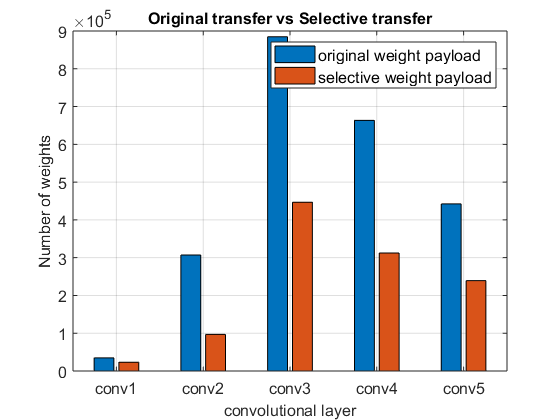
\includegraphics[width=2.5in]{Conv4bits}
\label{Con_Red}}
&
\subfloat[4bit weight, 1bit granularity]{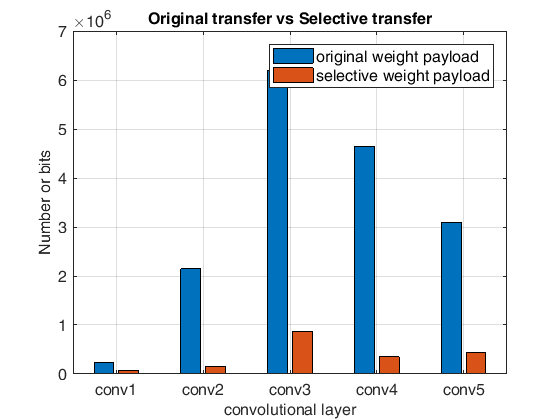
\includegraphics[width=2.5in]{Conv4bits_gran_bitlevel}
\label{Con_Red_bits}}
\\
\subfloat[8bit weight, 8bit granularity]{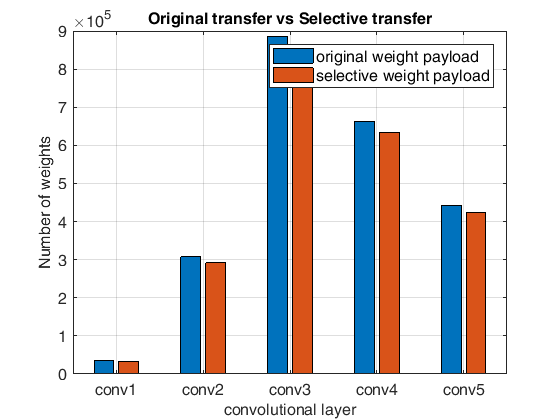
\includegraphics[width=2.5in]{Conv8bits} 
\label{Con_Red_8}}
&
\subfloat[8bit weight, 1bit granularity]{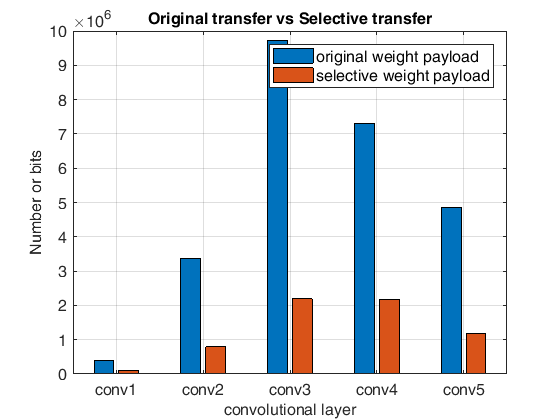
\includegraphics[width=2.5in]{Conv8bits_gran_bitlevel}
\label{Con_Red_8_bits}}\\ 
\end{tabular}
\caption{Redundancy analysis of the Convolutional Layer Weights}
\label{Conv_Red}

\begin{tabular}{cc}
\subfloat[4bit weights, 4bit granularity]{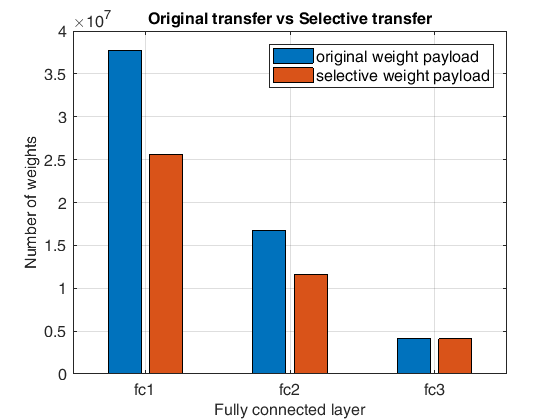
\includegraphics[width=2.5in]{FC4bits}
\label{FC_Red_4bits}}
&
\subfloat[4bit weights, 1bit granularity]{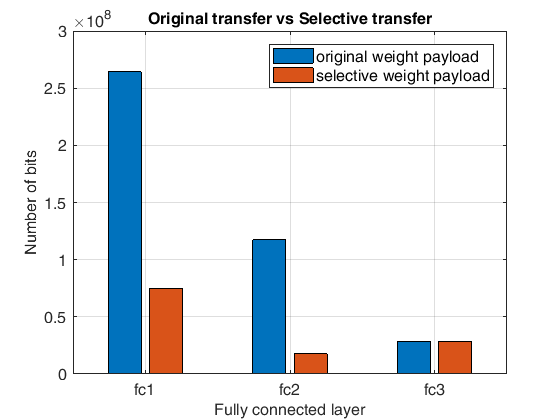
\includegraphics[width=2.5in]{FC4bits_gran_bitlevel}
\label{FC_Red_bits}}
\\
\subfloat[8bit weights, 8bit granularity]{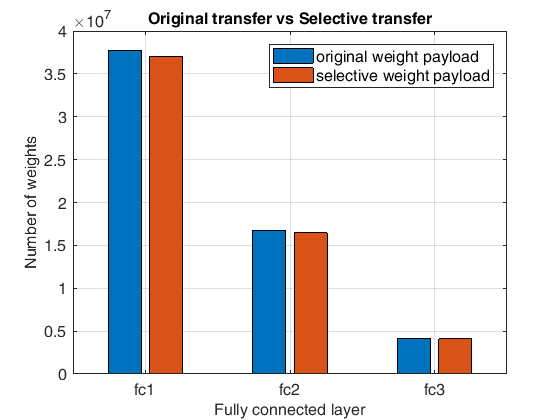
\includegraphics[width=2.5in]{FC8bits} 
\label{FC_Red_8bits_256lev}}
&
\subfloat[8bit weights, 1bit granularity]{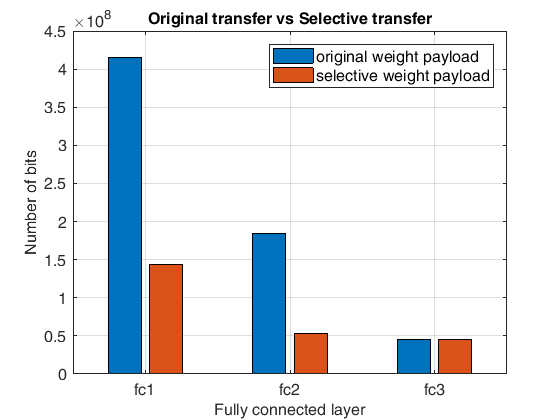
\includegraphics[width=2.5in]{FC8bits_gran_bitlevel} 
\label{FC_Red_8bits_256lev_bits}}\\ \\
\end{tabular}
\caption{Redundancy analysis of the Fully Connected Layer Weights}
\label{FC_Red}


\end{figure*}

\section{Design and Architecture}
The contribution of this paper lies in the main memory. We reuse the systolic architecture with nested processing elements we developed in \cite{Ansari_eff}.


\subsection{Processing in Memory}
Processing in memory or near data processing is done in a stacked DRAM. Stacked DRAM architectures are defined by \cite{standard2013high, black2013hybrid}. Each slice of DRAM is connected to each other with through silicon vias (TSVs). The DRAM is divided into smaller subsections called vaults. Each vertical vault is connected through and through, all the way to the logic layer. We implement the weight selector in the logic layer of the stacked DRAM. 
\begin{figure}[H]
\centering
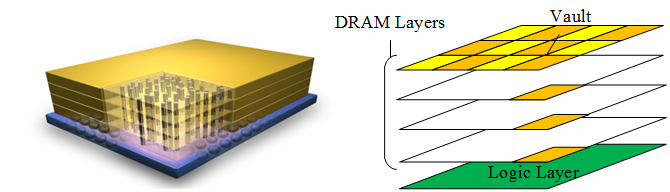
\includegraphics[width=3.5in]{HMC}
\caption{HMC model}
\label{HMC}
\end{figure}


\subsection{Weight Selector}

We incorporate the processing in memory DRAM architecture into our systolic array architecture we designed for \cite{Ansari_eff}. The main modification happens in the DRAM memory. The DRAM memory holds three kind of data payloads - input feature maps, filter weight kernel and output feature maps as described in figure \ref{arch}. Along with the data payloads mentioned earlier we house a weight selector unit inside the memory so as to only transfer fresh and different weight updates and not repeatedly send values that might be in the buffers already.This is described in figure \ref{WS}
\begin{figure}[!ht]
\centering
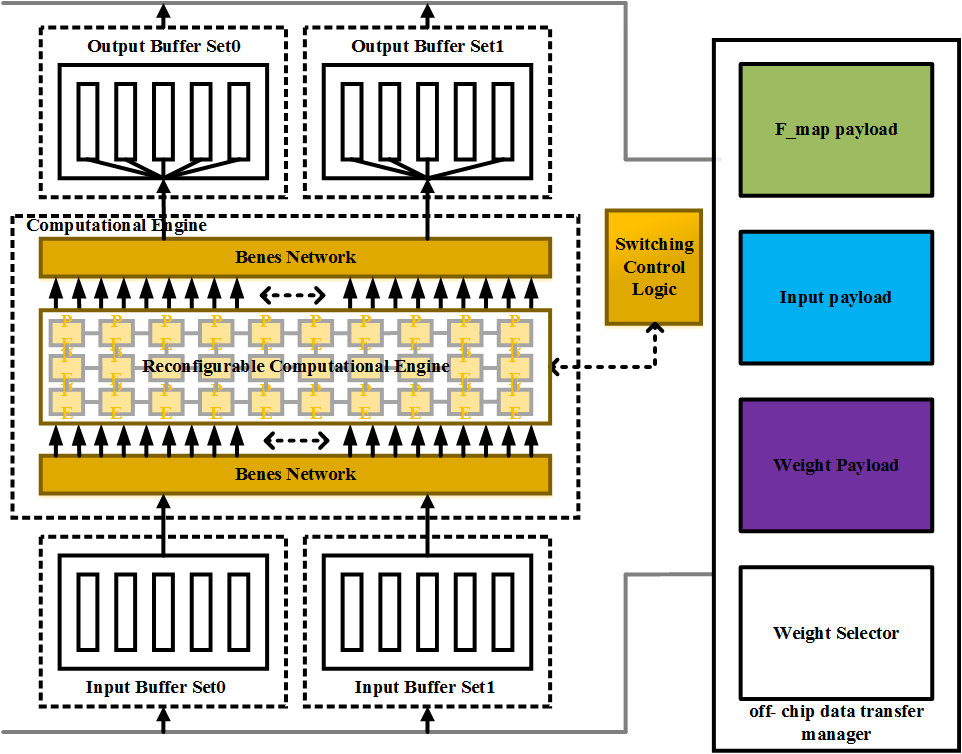
\includegraphics[width=3in]{arch}
\caption{Data Selector Architecture}
\label{arch}
\end{figure}


We have to deal with the latency of sending first batch of weights to the computation. Once the computation layer is initialized with weights we need to perform weight selection so that we send only new updated weight.

\begin{figure}[!ht]
\centering
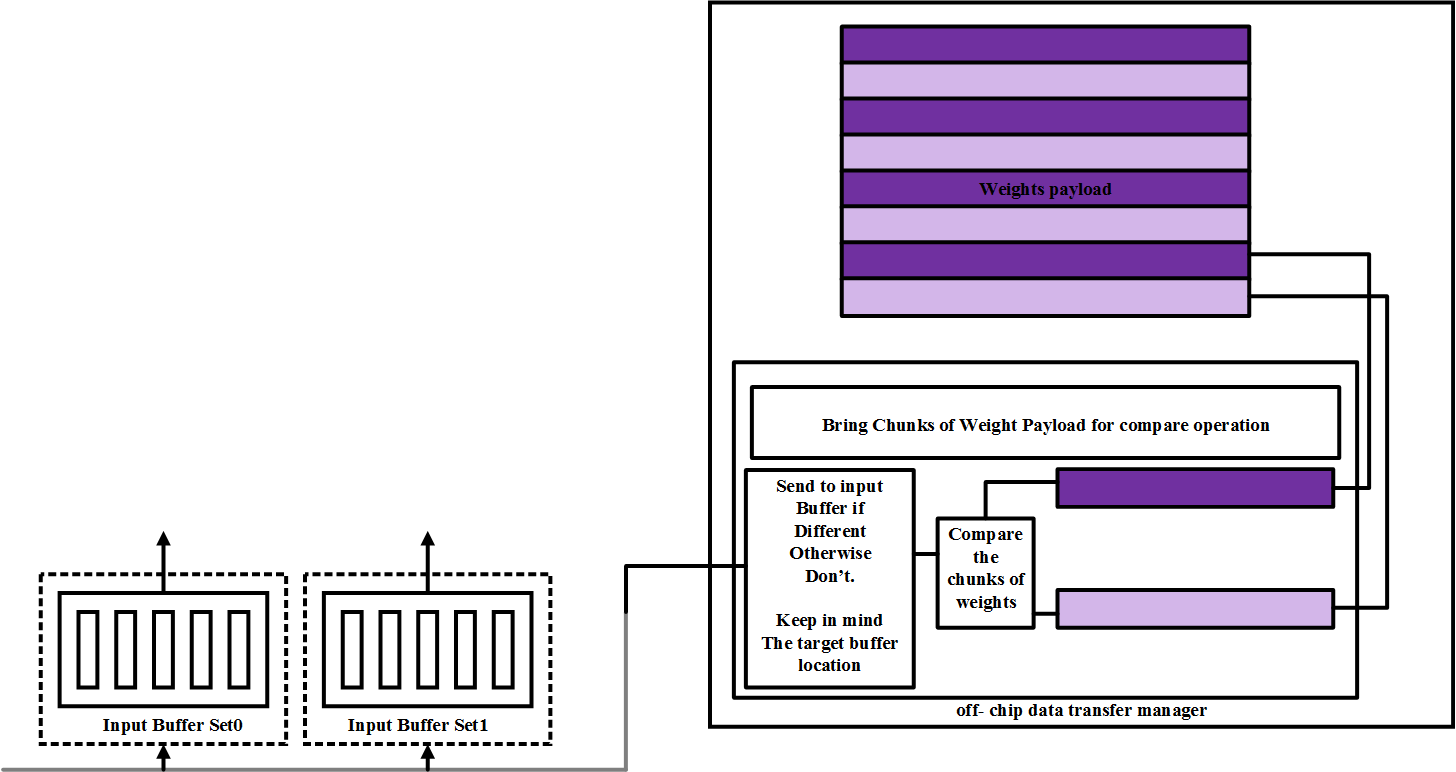
\includegraphics[width=3.5in]{WS}
\caption{Weight Selector Logic in DRAM}
\label{WS}
\end{figure}




%\subsubsection{FMap Selector}
%So many weights, 
%
%DeepCompression.
%
%
%
%
%Processing in Memory techniques. 


% no \IEEEPARstart


% You must have at least 2 lines in the paragraph with the drop letter
% (should never be an issue)


%\hfill mds
% 
%\hfill August 26, 2015

\section{Power Estimation}
The authors in \cite{energy_est_mit} have designed an online tool to estimate the energy consumption of DNN implementations using both computation and memory transfer cost. The values are normalized with respect to the energy cost of performing a MAC operation. We used the tool to estimate the energy consumption of the baseline AlexNet and the weight-sharing selective transfer AlexNet (WS-ST AlexNet). In figure \ref{Power_Est_1}, we see the energy consumption of the baseline AlexNet. In figure \ref{Power_Est_2}, we see the estimated power consumption of the weight-sharing selective transfer AlexNet. This power estimation is for both weight related computation cost and memory transfer. 

 

\begin{figure}[!ht]
\centering
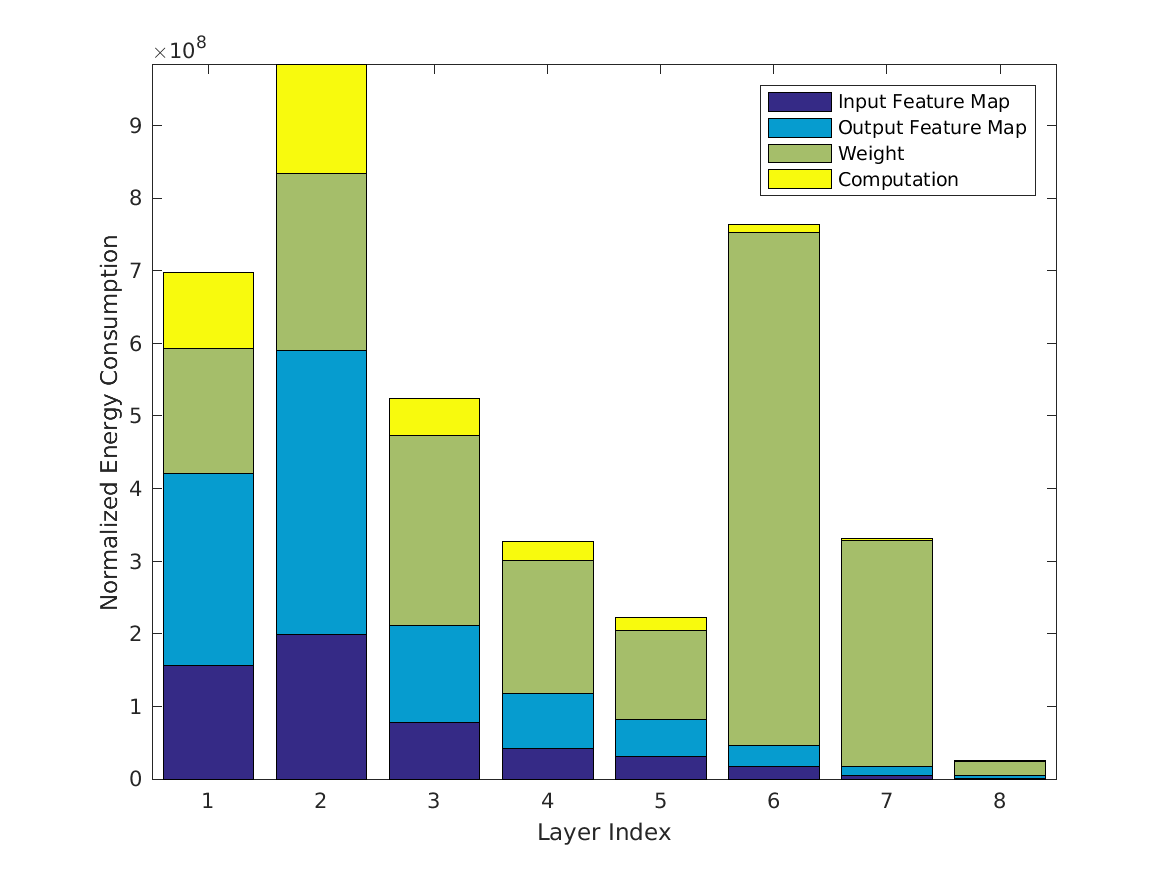
\includegraphics[width=2.5in]{EnergyVisualization_AlexNet}
\caption{Normalized Energy Consumption for AlexNet}
\label{Power_Est_1}
\end{figure}

\begin{figure}[!ht]
\centering
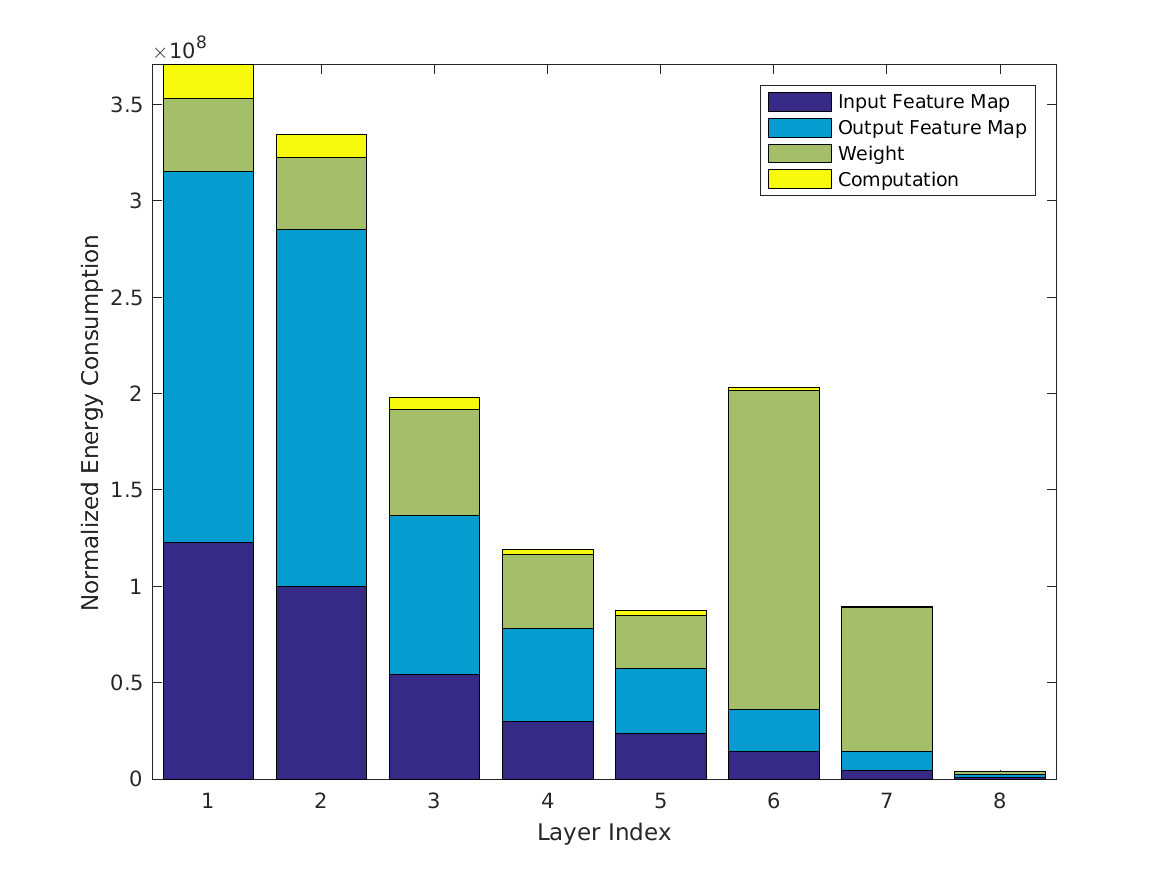
\includegraphics[width=2.5in]{EnergyVisualization_WSAlexNet}
\caption{Normalized Power Consumption for WS-ST AlexNet}
\label{Power_Est_2}
\end{figure}

The energy consumption just due to weights is described in figure \ref{Power_Est_3}. 

\begin{figure}[!ht]
\centering
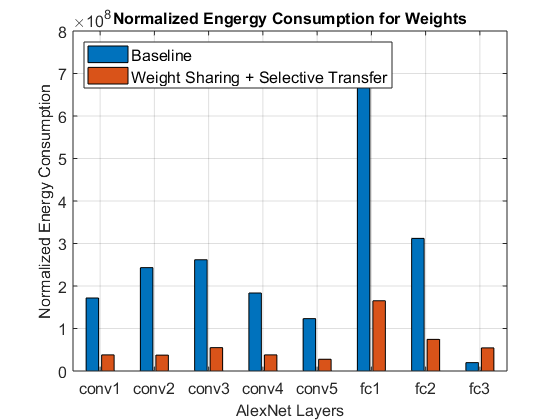
\includegraphics[width=2.5in]{Power_Est}
\caption{Normalized Power Consumption due to weights}
\label{Power_Est_3}
\end{figure}

\section{HDL Implementation}
We design a baseline DRAM and the WS-ST DRAM in Vivado and implement a design for the Virtex 7 family of devices. The results below in tables \ref{DPSP} and \ref{LogIO} are from those implementations. We can see there is a saving in WS-ST dynamic and static power. If we probe further, we can see that the Logic power and IO power that constitute the dynamic power also see a reducing trend. 

The memory width requirements for all layers are different. Fully connected layers have a large number of parameters. In our research, we find that storing fully connected layer parameters is difficult in a continuous block ram. Using a large continuous RAM increases the temperature of our target device to an unacceptable level during synthesis and implementation. 

WS-ST architecture is not the best solution for fully connected layers. We will need to compress the fully connected layers weights using some other form of compression. This brings forward the need for a hybrid technique for convolutional layer processing and fully connected layer processing. 

\begin{table}[!ht]
\centering
\caption{Dynamic Power (DP) and Static Power (SP) for Baseline AlexNet and WS-ST AlexNet in Watts}
\label{DPSP}
\begin{tabular}{ccccccc}
\hline
               & \multicolumn{2}{c}{\textbf{Baseline}}          & \multicolumn{2}{c}{\textbf{Selective}}         & \multicolumn{2}{c}{\textbf{\% Improvements}}   \\ 
\textbf{Layer} & \textbf{DP (W)} & \textbf{SP (W)} & \textbf{DP (W)} & \textbf{SP (W)} & \textbf{DP} & \textbf{SP} \\ \hline
\textbf{conv1} & 2.40                   & 0.26                  & 2.33                   & 0.26                  & 2.75                   & 0.00                  \\
\textbf{conv2} & 2.40                   & 0.26                  & 2.33                   & 0.26                  & 2.75                   & 0.00                  \\
\textbf{conv3} & 3.51                   & 0.28                  & 3.43                   & 0.28                  & 2.17                   & 0.36                  \\
\textbf{conv4} & 4.62                   & 0.30                  & 4.55                   & 0.29                  & 1.45                   & 0.34                  \\
\textbf{conv5} & 3.56                   & 0.28                  & 3.59                   & 0.28                  & -0.87                  & -0.36                 \\ \hline
\end{tabular}
\end{table}

\begin{table}[!ht]
\centering
\caption{Logic and IO power for Baseline AlexNet and WS-ST AlexNet in Watts }
\label{LogIO}
\begin{tabular}{ccccccc}
\hline
               & \multicolumn{2}{c}{\textbf{Baseline}} & \multicolumn{2}{c}{\textbf{Selective}} & \multicolumn{2}{c}{\textbf{\% Improvements}} \\ 
\textbf{Layer} & \textbf{IO (W)}               &\textbf{ Logic, (W)}             &\textbf{IO (W)}                  & \textbf{ Logic, (W)}            & \textbf{IO }                                   & \textbf{ Logic}  \\ \hline
\textbf{conv1} & 1.788             & 0.016             & 1.684              & 0.031             & 5.82                 & 0                     \\
\textbf{conv2} & 1.788             & 0.016             & 1.684              & 0.031             & 5.82                 & 0                     \\
\textbf{conv3} & 1.844             & 0.164             & 1.749              & 0.163             & 5.15                 & 0                     \\
\textbf{conv4} & 1.844             & 0.178             & 1.749              & 0.193             & 5.15                 & 0                     \\
\textbf{conv5} & 1.69              & 0.104             & 1.602              & 0.128             & 5.21                 & 0                     \\ \hline
\end{tabular}
\end{table}

\section{Results and Conclusion}
We achieve a $30\%$ reduction in the memory transfer of weights and $ 2\%$ saving in dynamic power due to weights for AlexNet. Similar reduction could be observed in other popular networks. The fully connected layers really raise the energy consumption of the device thus we will require to formulate a new technique to store the fully connected layer parameters.
In order to have a symmetry in architecture we will also need to implement a selection scheme on the output of the CNN layers. This will help us improve the offload  data write and read to the main memory. Thus contributing to the overall of reduction in memory transfer traffic and consequentially a reduction in energy consumption. 
% Please add the following required packages to your document preamble:






% An example of a floating figure using the graphicx package.
% Note that \label must occur AFTER (or within) \caption.
% For figures, \caption should occur after the \includegraphics.
% Note that IEEEtran v1.7 and later has special internal code that
% is designed to preserve the operation of \label within \caption
% even when the captionsoff option is in effect. However, because
% of issues like this, it may be the safest practice to put all your
% \label just after \caption rather than within \caption{}.
%
% Reminder: the "draftcls" or "draftclsnofoot", not "draft", class
% option should be used if it is desired that the figures are to be
% displayed while in draft mode.
%
%\begin{figure}[!t]
%\centering
%\includegraphics[width=2.5in]{myfigure}
% where an .eps filename suffix will be assumed under latex, 
% and a .pdf suffix will be assumed for pdflatex; or what has been declared
% via \DeclareGraphicsExtensions.
%\caption{Simulation results for the network.}
%\label{fig_sim}
%\end{figure}

% Note that the IEEE typically puts floats only at the top, even when this
% results in a large percentage of a column being occupied by floats.


% An example of a double column floating figure using two subfigures.
% (The subfig.sty package must be loaded for this to work.)
% The subfigure \label commands are set within each subfloat command,
% and the \label for the overall figure must come after \caption.
% \hfil is used as a separator to get equal spacing.
% Watch out that the combined width of all the subfigures on a 
% line do not exceed the text width or a line break will occur.
%
%\begin{figure*}[!t]
%\centering
%\subfloat[Case I]{\includegraphics[width=2.5in]{box}%
%\label{fig_first_case}}
%\hfil
%\subfloat[Case II]{\includegraphics[width=2.5in]{box}%
%\label{fig_second_case}}
%\caption{Simulation results for the network.}
%\label{fig_sim}
%\end{figure*}
%
% Note that often IEEE papers with subfigures do not employ subfigure
% captions (using the optional argument to \subfloat[]), but instead will
% reference/describe all of them (a), (b), etc., within the main caption.
% Be aware that for subfig.sty to generate the (a), (b), etc., subfigure
% labels, the optional argument to \subfloat must be present. If a
% subcaption is not desired, just leave its contents blank,
% e.g., \subfloat[].


% An example of a floating table. Note that, for IEEE style tables, the
% \caption command should come BEFORE the table and, given that table
% captions serve much like titles, are usually capitalized except for words
% such as a, an, and, as, at, but, by, for, in, nor, of, on, or, the, to
% and up, which are usually not capitalized unless they are the first or
% last word of the caption. Table text will default to \footnotesize as
% the IEEE normally uses this smaller font for tables.
% The \label must come after \caption as always.
%
%\begin{table}[!t]
%% increase table row spacing, adjust to taste
%\renewcommand{\arraystretch}{1.3}
% if using array.sty, it might be a good idea to tweak the value of
% \extrarowheight as needed to properly center the text within the cells
%\caption{An Example of a Table}
%\label{table_example}
%\centering
%% Some packages, such as MDW tools, offer better commands for making tables
%% than the plain LaTeX2e tabular which is used here.
%\begin{tabular}{|c||c|}
%\hline
%One & Two\\
%\hline
%Three & Four\\
%\hline
%\end{tabular}
%\end{table}


% Note that the IEEE does not put floats in the very first column
% - or typically anywhere on the first page for that matter. Also,
% in-text middle ("here") positioning is typically not used, but it
% is allowed and encouraged for Computer Society conferences (but
% not Computer Society journals). Most IEEE journals/conferences use
% top floats exclusively. 
% Note that, LaTeX2e, unlike IEEE journals/conferences, places
% footnotes above bottom floats. This can be corrected via the
% \fnbelowfloat command of the stfloats package.


%\section{Conclusion}


%\section{Future Work}





% trigger a \newpage just before the given reference
% number - used to balance the columns on the last page
% adjust value as needed - may need to be readjusted if
% the document is modified later
%\IEEEtriggeratref{8}
% The "triggered" command can be changed if desired:
%\IEEEtriggercmd{\enlargethispage{-5in}}

% references section

% can use a bibliography generated by BibTeX as a .bbl file
% BibTeX documentation can be easily obtained at:
% http://mirror.ctan.org/biblio/bibtex/contrib/doc/
% The IEEEtran BibTeX style support page is at:
% http://www.michaelshell.org/tex/ieeetran/bibtex/
\bibliographystyle{IEEEtran}
% argument is your BibTeX string definitions and bibliography database(s)
\bibliography{IEEEabrv,references}
%
% <OR> manually copy in the resultant .bbl file
% set second argument of \begin to the number of references
% (used to reserve space for the reference number labels box)
%\begin{thebibliography}{1}
%
%\bibitem{IEEEhowto:kopka}
%H.~Kopka and P.~W. Daly, \emph{A Guide to \LaTeX}, 3rd~ed.\hskip 1em plus
%  0.5em minus 0.4em\relax Harlow, England: Addison-Wesley, 1999.
%
%\end{thebibliography}




% that's all folks
\end{document}


